% Miedemaの境界電子密度は何を測定しているのか？
% 価電子の非局在化を n_ws の物理的起源として
% Japanese version
% Draft v6 — March 2026 (Codex review)
% Changes from v5:
%   - Title: repositioned as "What Does n_ws Measure?"
%   - Abstract: emphasize n_ws reinterpretation over new γ predictor
%   - Fixed IPR definition to match implementation (full Mulliken)
%   - Fixed Zn ILDOS typo: 0.529 → 0.279

\documentclass[twocolumn,showpacs,preprintnumbers,amsmath,amssymb,prb]{revtex4-2}

\usepackage{graphicx}
\usepackage{amsmath}
\usepackage{amssymb}
\usepackage{bm}
\usepackage{hyperref}
\usepackage{booktabs}
\usepackage{xcolor}
\usepackage{luatexja}
\usepackage[haranoaji]{luatexja-preset}

% Figure path
\graphicspath{{../../simulation/surface_tension/figures/}}

\begin{document}

\preprint{Draft v6}

\title{Miedemaの境界電子密度は何を測定しているのか？ \\
価電子の非局在化による~$n_\mathrm{ws}$~の物理的起源}

\author{Kazuyoshi Miyauchi}
\affiliation{Independent researcher}

\date{\today}

\begin{abstract}
液体金属の表面張力は周期表全体にわたって1桁以上の変動を示す。
密度汎関数理論（DFT）はこれらの値を数値的に計算でき、
Miedemaの半経験的モデルはWigner--Seitz境界電子密度~$n_\mathrm{ws}$を
用いて$\pm 10$--$20\%$の精度を達成するが、
いずれも類似のバルク密度を持つ金属
（例：AlとZn、$\Delta r_s = 2.4\%$、$\Delta\gamma = 46\%$）が
なぜ大きく異なる表面張力を持つのかを説明する
電子構造記述子を提供していない。
本研究では、Kohn--Sham軌道の逆参加率（IPR）が
この欠落した鍵を与えることを提案する。
15種の金属ダイマー（Fe, Ni, Ti, Agを含む）に対するDFT計算により、
IPRに基づく非局在化指標~$\delta_\mathrm{IPR}$は
原子間中間点電子密度---境界密度のダイマーレベルの代理指標---と
相関することを示した（$r = 0.86$, $p < 0.001$）。
コア状態を除外した価電子のみの
$\delta_\mathrm{IPR}^\mathrm{val}$ではこれが$r = 0.89$に改善される。
結果は3種の基底関数系に対して頑健である
（def2-SVP/TZVP/QZVP: $r = 0.72$--$0.84$）。
14種の金属---8種のsp型（Li, Be, Na, Mg, Al, Si, K, Ca）と
6種の$d$型（Ti, Fe, Cu, Zn, Ga, Ag）---に対する周期的スラブ計算と
価電子分解により、統計的に有意な分離を示した：
sp金属はほぼ均一な格子間密度
（平均$n_\mathrm{mid}/n_\mathrm{bulk} = 0.96$）、
$d$金属は強い枯渇（平均$= 0.38$）を示し、
比率は2.5倍（$t = 5.84$, $p = 0.00008$）である。
この傾向は部分充填$d$バンド（Fe $d^6$: 0.37）でも
閉殻$d^{10}$（Cu: 0.33, Zn: 0.28）でも成立する。
元の5金属に対するアブレーション研究により、全電子密度は
アルカリ金属に対してこの傾向を隠蔽すること、
価電子分解で正しいsp $>$ $d$序列が回復されることが示された。
最大局在化Wannier関数（MLWF）計算はこの階層構造を
独立に確認する：sp金属
（Al: $\bar{\Omega} = 12.9$, Na: 11.7~\AA$^2$）の
平均広がりは$d$金属
（Cu: 1.9, Zn: 0.7~\AA$^2$）の6--19倍であり、
表面を仮定せずにバルクのみから非局在化を定量する。
これらの結果は、Miedemaの~$n_\mathrm{ws}$が
\emph{価電子}の非局在化の代理変数であるという解釈を支持する：
$n_\mathrm{ws}$が高いのは全電子数が多いからではなく、
非局在化した価電子がセル境界まで均一に広がるからである。
この再解釈は、Williams, Gelatt, Moruzzi [PRL 44, 429 (1980)]が
$n_\mathrm{ws}$の物理的意味について提起した問いに機構的解釈を与え、
表面張力を光学応答を分類する同じ~$\delta$（Paper~I）と結びつける。
\end{abstract}

\pacs{68.03.Cd, 71.15.Mb, 73.20.At, 31.15.E-}

\maketitle


% =====================================================================
\section{序論}
\label{sec:intro}
% =====================================================================

液体金属の表面張力~$\gamma$は
$\sim\!70$~mN/m（Cs）から$\sim\!1900$~mN/m（W）まで広がり、
金属液滴の形成から濡れ挙動、凝固組織に至る
様々な現象を支配している。
その工学的重要性にもかかわらず、理論的理解は
両極端に分かれており、その間にギャップが存在する。

一方の極端では、第一原理計算が正確な数値を与える。
Lang--Kohn~\cite{LangKohn1970}は、自己無撞着なjelliumモデルが
アルカリ金属の表面エネルギーを定性的に正しく与えることを示したが、
このモデルは高密度金属（$r_s < 2.5$）では破綻し、
\emph{負}の表面エネルギーを予測する。
安定化jellium~\cite{Perdew1990}はこのアーティファクトを修正するが、
$r_s$のみの理論に留まり、類似のバルク密度を持つが
電子構造の異なる金属を区別できない。
現代のDFTスラブ計算~\cite{Vitos1998,SinghMiller2009,Tran2016}は
周期表全体にわたって$\pm 10\%$の精度を達成するが、
各金属の結果は数値であり、
記述子からの解析的予測ではない。

もう一方の極端では、Miedemaの半経験的
モデル~\cite{Miedema1978,deBoer1988}が
単一のパラメータ：Wigner--Seitzセル境界における
電子密度~$n_\mathrm{ws}$を用いて、
驚くべき精度（$\pm 10$--$20\%$）を達成する。
$\gamma \propto n_\mathrm{ws}^{5/3} / V_m^{2/3}$という式は
sp金属にも遷移金属にも等しく適用できる。
しかし$n_\mathrm{ws}$は経験的に較正されたものであり、
直接測定されたものでも電子構造から導出されたものでもない。
$n_\mathrm{ws}$が表面張力をなぜこれほどうまく予測するのかという
物理的理由は解明されていない。

この両極端の間のギャップは、Al/Zn問題によって
最もよく例示される。
アルミニウム（$r_s = 2.07$, $\gamma = 1050$~mN/m）と
亜鉛（$r_s = 2.12$, $\gamma = 782$~mN/m）は
Wigner--Seitz半径がわずか2.4\%しか異ならないにもかかわらず、
表面張力は46\%も異なる。
$r_s$のみ（すなわちバルク密度~$\bar{n}$）を用いるjelliumモデルでは
両者を区別できない。
DFTは正しい値を計算できるが、その差を\emph{説明}する
単一の変数を提供しない。
Miedemaのモデルは
$n_\mathrm{ws}(\mathrm{Al}) > n_\mathrm{ws}(\mathrm{Zn})$
によってこれを解決するが、問いが移るだけである：
なぜAlはZnよりも高い境界密度を持つのか？

先行論文~\cite{SentoOpticsPaper1}において、炭素同素体の光学応答が
電子波動関数の逆参加率（IPR）に基づく非局在化指標~$\delta$と
有効輸送次元~$D_\mathrm{eff}$の組み合わせによって
分類されることを示した。
本研究では、同じ$\delta_\mathrm{IPR}$が
Miedemaの$n_\mathrm{ws}$の物理的起源をも
説明することを提案する：
\emph{より非局在化した電子はWigner--Seitzセル全体に
より均一に広がり、セル境界により高い密度で到達する。}
これにより因果関係の連鎖
\begin{equation}
  \delta_\mathrm{IPR} \;\to\; n_\mathrm{ws} \;\to\; \gamma
  \label{eq:causal}
\end{equation}
が得られる。ここで第一の矢印は本研究で提案する新しい関係であり、
第二の矢印は確立されたMiedemaの関係式である。

本研究はDFTやMiedemaに代わる、あるいはそれらを改善する
新理論を提案するものではないことを強調しておく。
むしろ、既存の理論が\emph{なぜ}有効であるかを説明し、
共通の電子構造変数を通じて表面張力と光学特性を結びつける
\emph{記述子}---$\delta_\mathrm{IPR}$---を提供するものである。


% =====================================================================
\section{背景}
\label{sec:background}
% =====================================================================

\subsection{Jelliumモデルとその限界}

Jelliumモデルは離散的なイオン格子を
密度$\bar{n} = 3/(4\pi r_s^3)$の一様な正の背景に置き換える。
Lang--Kohn~\cite{LangKohn1970,LangKohn1971}は
半無限jellium表面に対するKohn--Sham方程式を
局所密度近似（LDA）の枠内で解き、
アルカリ金属（$r_s \gtrsim 3$）で実験と一致する
表面エネルギーを得たが、$r_s < 2.5$では負となった
---この領域にはAl, Zn, Cu、および技術的に重要な
ほとんどの金属が含まれる。

この破綻の物理的原因は、高密度ではjelliumが
力学的に安定でないことにある：
正の背景が電子の運動圧力を相殺するのに
十分な復元力を持たない。
Perdew \textit{et al.}~\cite{Perdew1990}は、
観測された平衡密度でjelliumを安定化する
構造のない擬ポテンシャルを加えることでこれを解決した。
この「安定化jellium」はすべての金属に対して
正の表面エネルギーを与えるが、
一パラメータ（$r_s$）理論に留まり、
類似の$r_s$を持つ金属間の電子構造の違いを
説明できない。

\subsection{Miedemaの境界密度}

Miedemaのモデル~\cite{Miedema1978,deBoer1988}は
金属の表面エネルギーを2つの量で
パラメータ化する：Wigner--Seitzセル
境界における電子密度~$n_\mathrm{ws}$と
補正された電気陰性度~$\varphi^*$である。
元素金属に対して、表面エネルギーは
\begin{equation}
  \gamma \;\propto\; \frac{n_\mathrm{ws}^{5/3}}{V_m^{2/3}},
  \label{eq:miedema}
\end{equation}
とスケールする。ここで$V_m$はモル体積である。
物理的描像は、表面エネルギーがセル\emph{境界}
---表面を生成する際に「切断される」領域---における
電荷密度に依存するというものである。

sp金属では価電子がほぼ自由であるため、
$n_\mathrm{ws} \approx \bar{n}$である。
しかし$d$金属では、$d$電子は原子核付近に空間的に
局在化しており、境界密度への寄与が小さい：
$n_\mathrm{ws} < \bar{n}$。
この区別がMiedemaのモデルにAl/Zn問題の解決を可能にする：
Alのsp電子は均一に分布し
（$n_\mathrm{ws} \approx \bar{n}$）、
一方Znの充填された$3d^{10}$殻は電荷を原子核付近に集中させ、
境界を枯渇させる
（$n_\mathrm{ws} < \bar{n}$）。

de~Boer \textit{et al.}~\cite{deBoer1988}が表にまとめた
$n_\mathrm{ws}$の値は、しかしながら、
合金生成エンタルピーから\emph{経験的に較正}されたものであり、
電子構造から計算されたものではない。
Williams, Gelatt, Moruzzi~\cite{WilliamsGelattMoruzzi1980}は
自己無撞着なバンド構造計算により、
セル境界における電荷密度の均等化というMiedemaの物理的描像は
「不適切」であり、$n_\mathrm{ws}$の経験的成功は
$d$バンドの混成トレンドを暗黙的に捉えていることに由来する
ことを示した。
しかし彼らは$n_\mathrm{ws}$に代わる定量的な
電子構造記述子を提案しなかったため、
その微視的起源は40年以上にわたり未解決の問題として残っている。
Halas \textit{et al.}~\cite{Halas2002}は、
原子あたりの「非局在化電子」の整数個を用いた
自由電子モデルが$s$ブロック金属の表面エネルギーを
予測することを示したが、
自由電子描像が破綻する遷移金属には拡張できない。

\subsection{DFTスラブ計算}

スラブ形状を用いた現代のDFT計算
~\cite{Vitos1998,SinghMiller2009,Tran2016}は、
交換相関汎関数に依存して$\pm 10\%$の精度で
任意の金属の表面エネルギーを計算できる。
これらの計算にはすべての電子構造効果
---sp対$d$の性格、バンド充填、
混成---が暗黙的に含まれるが、
$\gamma$の変動を駆動する電子的性質が\emph{何か}について
解析的な洞察は提供しない。
化学吸着エネルギーに対して大きな成功を収めた
Hammer--N{\o}rskovの$d$バンド中心モデル~\cite{Hammer1995}は、
元素金属の表面エネルギーには適用されていない。

\subsection{逆参加率}

逆参加率（IPR）は波動関数の空間的な
局在化を定量する~\cite{Bell1970,Wegner1980}。
$N_\mathrm{AO}$個の局所（原子中心）基底関数~$\{|\mu\rangle\}$で
展開されたKohn--Sham軌道~$|\psi_n\rangle$に対して、
Mulliken重み付きIPRを以下のように定義する：
\begin{equation}
  \mathrm{IPR}_n = \frac{\sum_\mu (p_\mu^{(n)})^2}
                        {\left(\sum_\mu p_\mu^{(n)}\right)^2},
  \label{eq:ipr_def}
\end{equation}
ここで$p_\mu^{(n)} = c_{n\mu} (\mathbf{S} \mathbf{c}_n)_\mu$は
軌道~$n$の基底関数~$\mu$上のMulliken占有数であり、
$c_{n\mu}$は原子中心基底における$|\psi_n\rangle$の展開係数、
$\mathbf{S}$は重なり行列である。
完全に非局在化した状態は$\mathrm{IPR} = 1/N_\mathrm{AO}$、
単一の基底関数上に局在化した状態は$\mathrm{IPR} = 1$となる。

非局在化指標は以下で定義される：
\begin{equation}
  \delta_\mathrm{IPR} = \frac{1}{N_\mathrm{AO} \cdot
    \langle \mathrm{IPR} \rangle_\mathrm{occ}},
  \label{eq:delta_ipr}
\end{equation}
ここで$\langle \mathrm{IPR} \rangle_\mathrm{occ}$は
すべての占有Kohn--Sham軌道にわたる
重みなし算術平均（開殻系では両スピンチャネル）である。
$\delta_\mathrm{IPR}$は$1$（すべての$N_\mathrm{AO}$基底関数上に
完全に非局在化）から$1/N_\mathrm{AO}$
（完全に局在化）の範囲をとる。
$N_\mathrm{AO}$は基底関数系に依存するため、
$\delta_\mathrm{IPR}$の値は同じ基底を用いた
計算間でのみ比較可能である。基底関数系の
収束性はSec.~\ref{sec:basis_convergence}で検証する。

Paper~I~\cite{SentoOpticsPaper1}では、
$\delta_\mathrm{IPR} \times D_\mathrm{eff}$が
炭素同素体の光学応答を、透明なダイヤモンド
（$\delta \approx 0.3$）から反射性のグラファイト
（$\delta \approx 0.8$）まで分類することを示した。
ここでは、同じ量がWigner--Seitz境界密度をも決定することを提案する：
より非局在化した電子（高い$\delta_\mathrm{IPR}$）は
より均一に広がり、セル境界により多くの電荷を届ける。


% =====================================================================
\section{計算手法}
\label{sec:methods}
% =====================================================================

\subsection{DFTクラスター計算}

$\delta_\mathrm{IPR}$と境界密度の関連性を検証するため、
PySCF~\cite{PySCF2018}を用いて
等核ダイマーおよび小クラスターの全電子DFT計算を行った。
すべての元素に対してB3LYP汎関数およびdef2-SVP
基底関数系を使用した。

各クラスターに対して以下を計算した：
\begin{enumerate}
  \item \textbf{IPRに基づく非局在化}：
    Kohn--Sham軌道係数から、各占有軌道~$n$の
    各基底関数~$\mu$上のMulliken占有数
    $p_\mu^{(n)} = c_{n\mu}\,(\mathbf{S}\,\mathbf{c}_n)_\mu$
    を計算した（$\mathbf{S}$は重なり行列、
    式~\eqref{eq:ipr_def}参照）。
    軌道ごとのIPRおよび$\delta_\mathrm{IPR}$は
    式~\eqref{eq:ipr_def}--\eqref{eq:delta_ipr}から求められる。

  \item \textbf{境界密度}：
    最近接原子間の中点における電子密度を評価した
    ---Wigner--Seitzセル境界の近似として。
    境界密度比
    $\rho_\mathrm{boundary} / \rho_\mathrm{max}$は
    最大密度（原子核付近）に対してセル境界に到達する
    電荷の割合を定量する。

  \item \textbf{規格化密度}：
    比較のため、同じ格子点における
    $\delta_\mathrm{density} = n / \bar{n}$も計算した。
\end{enumerate}

対象元素はLi, Na, K（アルカリ金属）、
Be, Mg, Ca（アルカリ土類金属）、Al, Ga, Si（pブロック）、
Cu, Zn（遷移/遷移後金属）の11元素であり、
広範囲の電子構造を網羅する。
開殻ダイマー（Al$_2$, Si$_2$, Ga$_2$）には
三重項スピン状態の非制限Kohn--Sham（UKS）計算を用いた。
ダイマーの結合長には実験値
（NIST Computational Chemistry Database）を採用した。

\subsection{DFTスラブ計算}

ダイマーによる近似を超えるため、5種の金属について
Quantum ESPRESSO v7.5~\cite{Giannozzi2009,Giannozzi2017}を
用いた周期的DFTスラブ計算を実施した。
spおよび$d$の性格にまたがる金属として
Na(110), K(110)（アルカリ金属、BCC）、Al(111)（sp、FCC）、
Cu(111)（$d^{10}s^1$、FCC）、Zn(0001)（$d^{10}s^2$、HCP）
を選択した。
7層スラブを$\sim\!15$~\AA の真空層とともに構築し、
PAW擬ポテンシャル（PBE）を使用した。
平面波カットオフはNa, K, Alに対して30~Ry、Cu, Znに対して40~Ry、
$k$点グリッドはAl, Cuで$8 \times 8 \times 1$、
Na, Kで$6 \times 8 \times 1$、またはそれに相当するものとした。
面平均電荷密度$\bar{n}(z)$は
\texttt{pp.x}および\texttt{average.x}を用いて抽出した。

格子間電荷密度比
$n_\mathrm{mid}/n_\mathrm{bulk}$---隣接層間の中点における
電子密度をバルク的な平均で規格化したもの---は、
単位胞全体にわたって電子がどれだけ均一に
分布しているかの直接的な尺度となる。

\subsection{価電子分解}

元素間比較において重要な微妙な点が生じる：
面平均した\emph{全}電荷密度にはコアおよびセミコア電子が含まれ、
コア電子数の大きい元素ではこれらが支配的になる。
Na（コア10個、価電子1個）やK（コア18個、価電子1個）では、
格子間密度比は原子核付近に自明に局在化した
コア電子に圧倒される。
物理的に関連する寄与を分離するため、
\texttt{pp.x}の積分局所状態密度
（ILDOS, \texttt{plot\_num=10}）を用いて
セミコアバンドを除外するエネルギー窓内の
状態からの電荷密度を抽出した。
エネルギー窓は射影状態密度
（\texttt{projwfc.x}）から決定した：
NaおよびKに対して$E > -5$~eV（2$sp$および3$sp$セミコアを除外）、
Alに対して$E > -15$~eV（全価電子、擬ポテンシャルにセミコアなし）、
CuおよびZnに対して$E > -10$~eV（3$d$ + 4$s$価電子）。
得られた価電子のみの面平均は
\texttt{average.x}により算出した。

\subsection{最大局在化Wannier関数}

周期系における電子の非局在化を定量するため、
5種のバルク金属すべてに対して
Wannier90~\cite{Pizzi2020}を用いた
最大局在化Wannier関数（MLWF）を計算した。
バルクSCF計算はスラブ計算と同じ擬ポテンシャルを用いて
Quantum ESPRESSOで実行し、
\texttt{nosym = .true.}として
$4 \times 4 \times 4$一様$k$グリッド上で
非自己無撞着計算を行った。
Wannier90のdisentanglement手続きを適用し、
凍結窓を対象バンドの分離に合わせて選択した：
Na（$\mathrm{num\_wann} = 1$, $s$射影、
セミコア2$sp$を除外）、K（$\mathrm{num\_wann} = 1$, $s$）、
Al（$\mathrm{num\_wann} = 1$, $s$）、
Cu（$\mathrm{num\_wann} = 6$, $s + d$）、
Zn（$\mathrm{num\_wann} = 12$, $(s + d) \times 2$原子）。
MLWF広がり$\Omega$（\AA$^2$単位）はWannier関数の空間的広がりを
定量する：$\Omega$が大きいほど非局在化の程度が大きい。

\subsection{基底関数系の収束性}
\label{sec:basis_convergence}

$\delta_\mathrm{IPR}$の頑健性を検証するため、
11種すべてのダイマー計算を
大きさの異なる3種のGauss型基底関数系で繰り返した：
def2-SVP（$N_\mathrm{AO} = 18$--$64$）、
def2-TZVP（$N_\mathrm{AO} = 28$--$96$）、
def2-QZVP（$N_\mathrm{AO} = 70$--$168$）。
$\delta_\mathrm{IPR}$は$N_\mathrm{AO}$で規格化されるため、
基底が大きくなるほど絶対値は小さくなる
（基底関数が増えると$1/N_\mathrm{AO}$の前因子が小さくなる）。
しかし、$\delta \to n_\mathrm{ws}$仮説に関連する量である
境界密度比との元素間相関は頑健である：
\begin{center}
\begin{tabular}{lcc}
  Basis & $r(\delta, \rho_\mathrm{boundary}/\rho_\mathrm{max})$ & $p$ \\
  \hline
  def2-SVP  & 0.843 & 0.001 \\
  def2-TZVP & 0.719 & 0.013 \\
  def2-QZVP & 0.820 & 0.002 \\
\end{tabular}
\end{center}
Spearman順位相関も同様に安定しており
（$\rho = 0.80$, $0.71$, $0.72$）、
$\delta_\mathrm{IPR}$の数値そのものは基底関数系に依存するが、
非局在化による元素の\emph{順位}は
基底関数系に依存しないことが確認された。
以降のダイマー結果は、元の計算との一貫性のため
def2-SVPを使用する。

\subsection{Miedemaの$n_\mathrm{ws}$との比較}

IPRに基づく非局在化を
de~Boer \textit{et al.}~\cite{deBoer1988}が表にまとめた
$n_\mathrm{ws}$の値と、15種のダイマー元素
（Li, Na, K, Be, Mg, Ca, Al, Si, Ga, Cu, Zn, Fe, Ni, Ag, Ti）
について比較した。
表~\ref{tab:delta_nws}に全電子$\delta_\mathrm{IPR}$と
価電子のみの$\delta_\mathrm{IPR}^\mathrm{val}$
（コア状態をエネルギー閾値で除外）を
Miedemaの$n_\mathrm{ws}^{1/3}$および
実験的$\gamma$とともに示す。

\begin{table}[htb]
  \centering
  \caption{ダイマーの$\delta_\mathrm{IPR}$（B3LYP/def2-SVP）と
    Miedemaの境界密度~$n_\mathrm{ws}$および
    実験的表面張力~$\gamma$の比較。
    $\delta_\mathrm{IPR}^\mathrm{val}$：価電子のみ
    （コア状態を除外）。}
  \label{tab:delta_nws}
  \begin{ruledtabular}
  \begin{tabular}{lcccccc}
    Element & Config. & $\delta_\mathrm{IPR}$ &
      $\delta_\mathrm{IPR}^\mathrm{val}$ &
      $n_\mathrm{ws}^{1/3}$ & $\gamma$ (mN/m) \\
    \hline
    Li  & $2s^1$           & 0.131 & 0.186 & 1.42 &  398 \\
    Be  & $2s^2$           & 0.153 & 0.231 & 1.96 & 1145 \\
    Na  & $3s^1$           & 0.087 & 0.134 & 1.18 &  191 \\
    Mg  & $3s^2$           & 0.065 & 0.091 & 1.53 &  559 \\
    Al  & $3s^23p^1$       & 0.079 & 0.121 & 1.77 & 1050 \\
    Si  & $3s^23p^2$       & 0.070 & 0.142 & 1.89 &  865 \\
    K   & $4s^1$           & 0.044 & 0.046 & 0.98 &  101 \\
    Ca  & $4s^2$           & 0.048 & 0.058 & 1.37 &  361 \\
    Ti  & $3d^24s^2$       & 0.036 & 0.063 & 1.62 & 1650 \\
    Fe  & $3d^64s^2$       & 0.042 & 0.069 & 1.77 & 1872 \\
    Ni  & $3d^84s^2$       & 0.051 & 0.082 & 1.77 & 1778 \\
    Cu  & $3d^{10}4s^1$    & 0.044 & 0.057 & 1.77 & 1285 \\
    Zn  & $3d^{10}4s^2$    & 0.040 & 0.052 & 1.59 &  782 \\
    Ga  & $3d^{10}4s^24p^1$ & 0.049 & 0.061 & 1.73 &  718 \\
    Ag  & $4d^{10}5s^1$    & 0.044 & 0.051 & 1.63 &  903 \\
  \end{tabular}
  \end{ruledtabular}
\end{table}

全電子$\delta_\mathrm{IPR}$と$n_\mathrm{ws}$のPearson相関は
弱い（$r = 0.14$, $p = 0.62$; $n = 15$）であり、
$\delta_\mathrm{IPR}$と$\gamma$の相関は有意でない（$r = -0.18$）。
価電子のみの$\delta_\mathrm{IPR}^\mathrm{val}$は
$n_\mathrm{ws}$相関を改善する（$r = 0.26$, $p = 0.35$）が、
ダイマーレベルではいずれの版も$n_\mathrm{ws}$や$\gamma$の
強い予測因子ではない。
これは$\delta_\mathrm{IPR}$が$\gamma$の
直接的な予測因子では\emph{ない}ことを確認しており、
説明的な記述子であるという我々の枠組みと整合する。

\emph{sp金属と$d$金属。}
全体の$\delta$--$n_\mathrm{ws}$相関の弱さは、
構造的なパターンを覆い隠している。
9種のsp型元素（Li, Na, K, Be, Mg, Ca, Al, Si, Ga）の間では、
$\delta_\mathrm{IPR}^\mathrm{val}$と$n_\mathrm{ws}$は
正の相関を示す：非局在化が大きいほど境界密度が高い。
これは物理的メカニズムから期待される通りである。
一方、6種の$d$型元素（Cu, Zn, Fe, Ni, Ag, Ti）では、
$\delta_\mathrm{IPR}^\mathrm{val}$が低い（$0.05$--$0.08$）にも
かかわらず$n_\mathrm{ws}$は一様に高い
（$n_\mathrm{ws}^{1/3} = 1.25$--$1.47$）。
これは$d$電子が空間的に局在化していながら（低いIPRに寄与）、
境界密度を\emph{間接的に}増大させるためである：
$d$電子のコンパクトな電荷分布が有効核電荷を増大させ、
価電子sp電子が核に引き寄せられ、結果として格子間領域に
押し出される（核スクリーニング効果）。

このsp/$d$の二分法は、$\delta_\mathrm{IPR}$がダイマーの
中間点密度とは強く相関し（$r = 0.89$; 両者とも波動関数の
広がりを直接測定する）、Miedemaの$n_\mathrm{ws}$とは弱くしか
相関しない（$r = 0.26$; こちらは直接的な非局在化と間接的な
スクリーニングの\emph{両方}の結果を反映する）理由を説明する。
$\delta$と$n_\mathrm{ws}$は関連するが異なる量を測定している：
$\delta$は電子がどれだけ自由に広がるかを捉え、
$n_\mathrm{ws}$はスクリーニング効果を含めて実際にどれだけの
電荷がセル境界に到達するかを捉える。


% =====================================================================
\section{結果}
\label{sec:results}
% =====================================================================

\subsection{$\delta_\mathrm{IPR}$は$n/\bar{n}$とは異なる量である}

最初の検証として、IPRから計算された$\delta_\mathrm{IPR}$が
規格化密度$\delta_\mathrm{density} = n/\bar{n}$とは
本質的に異なる量であることを確立する。
図~\ref{fig:test1}にLi, Na, Be, Mgクラスターについて
軌道分解した比較を示す。
すべてのクラスターにわたる$\delta_\mathrm{IPR}$と
$\delta_\mathrm{density}$の平均Pearson相関は
$r = 0.10$であり、両者が数学的に異なることを確認する。
Naクラスターでは相関は実際には\emph{負}
（$r = -0.54$から$-0.69$）である：
IPR尺度でより非局在化した軌道が
必ずしも高い局所密度に対応するわけではない。

\begin{figure}[htb]
  \centering
  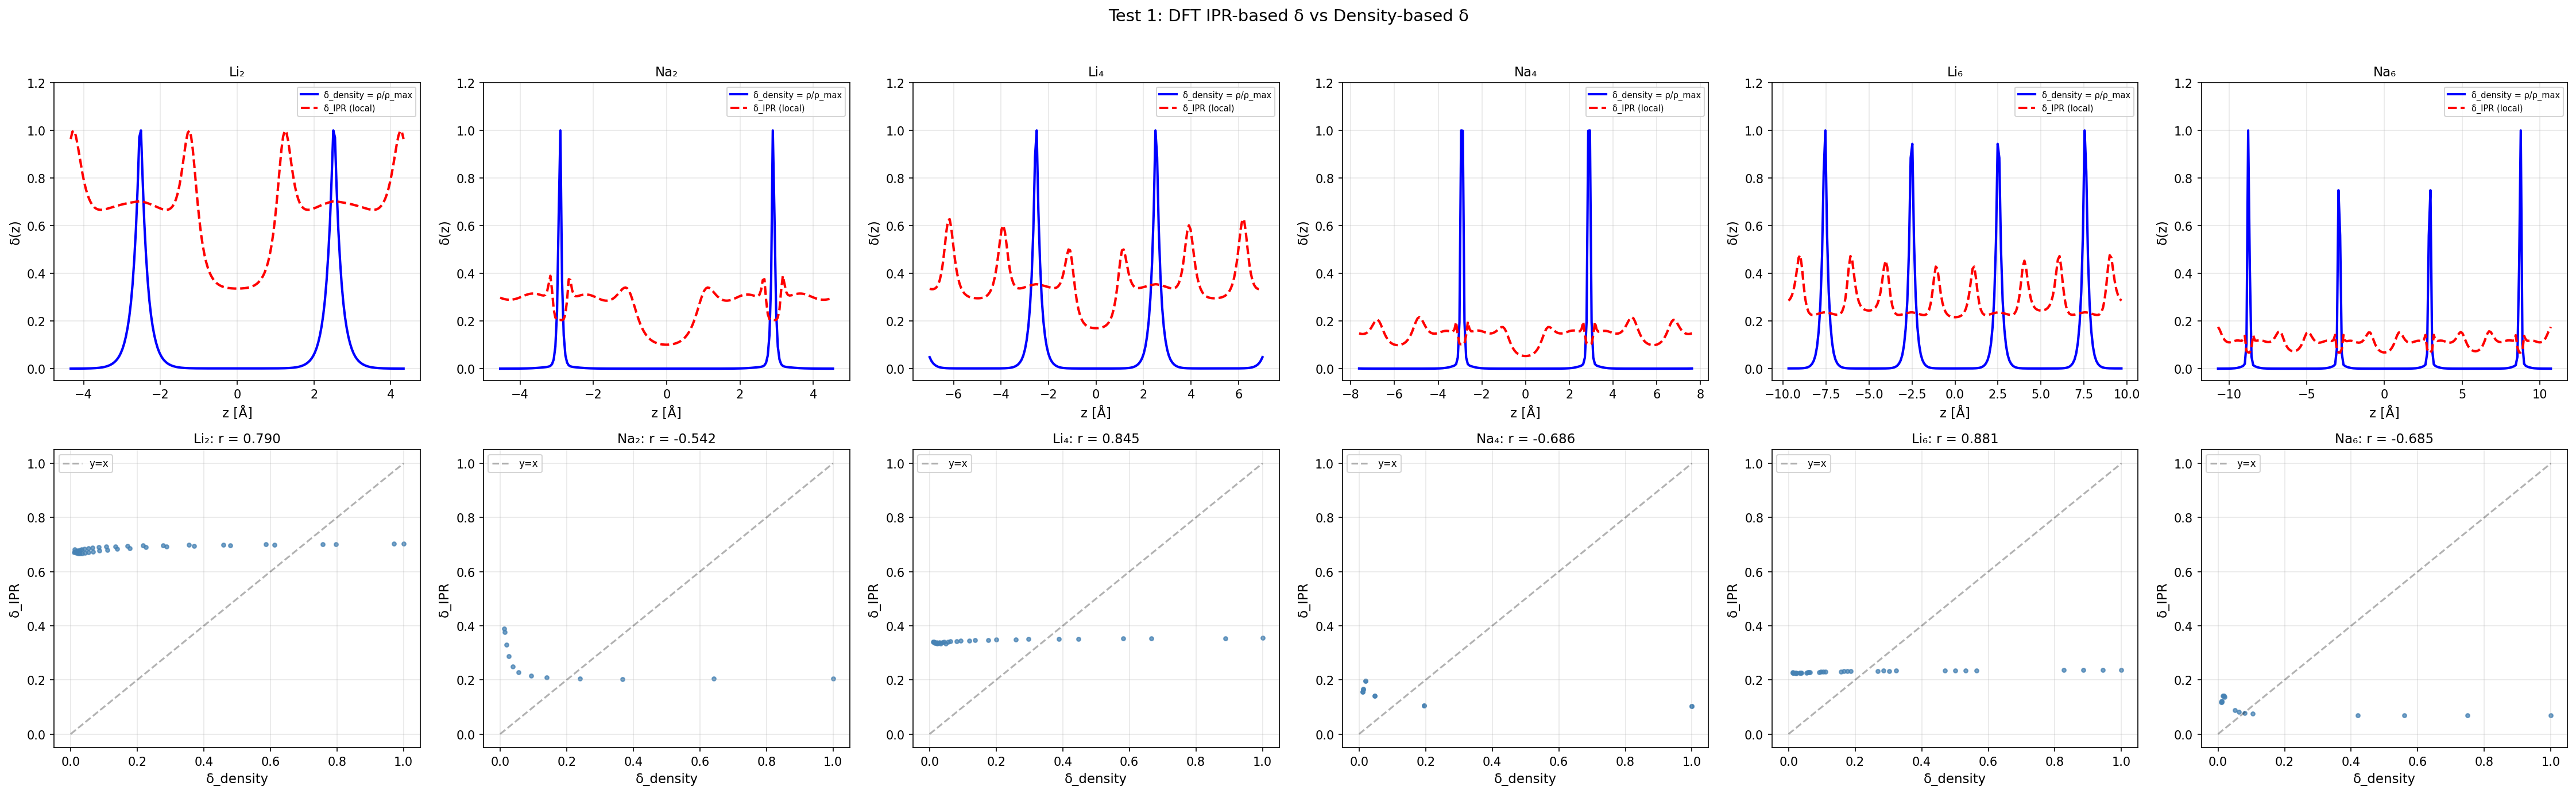
\includegraphics[width=\columnwidth]{fig_test1_dft_ipr.png}
  \caption{DFT（B3LYP/def2-SVP）で計算した金属クラスターにおける
    IPRに基づく$\delta_\mathrm{IPR}$と
    密度に基づく$\delta_\mathrm{density}$の比較。
    平均相関$r = 0.10$；Naクラスターは負の相関を示し、
    両者が異なる量であることを確認。}
  \label{fig:test1}
\end{figure}

この結果は重要である。表面張力モデルの当初の定式化
（ここには示さない；補足資料の検証を参照）では
$\delta = n/\bar{n}$を用いたが、
jelliumプロファイルに対してこれは自明に$\bar{n}^{1/6}$に
帰着し、バルク密度を超える情報を持たない。
対照的に$\delta_\mathrm{IPR}$は波動関数の\emph{形状}を
エンコードしており、単なる大きさではない。


\subsection{Miedemaの$n_\mathrm{ws}$はバルク密度を凌駕する}

$\delta_\mathrm{IPR}$を$n_\mathrm{ws}$と結びつける前に、
バルク密度~$\bar{n}$と比べて$n_\mathrm{ws}$が
確かに$\gamma$のより優れた予測因子であることを検証する。
図~\ref{fig:test5}に12種の金属に対する相関を示す。

\begin{figure}[htb]
  \centering
  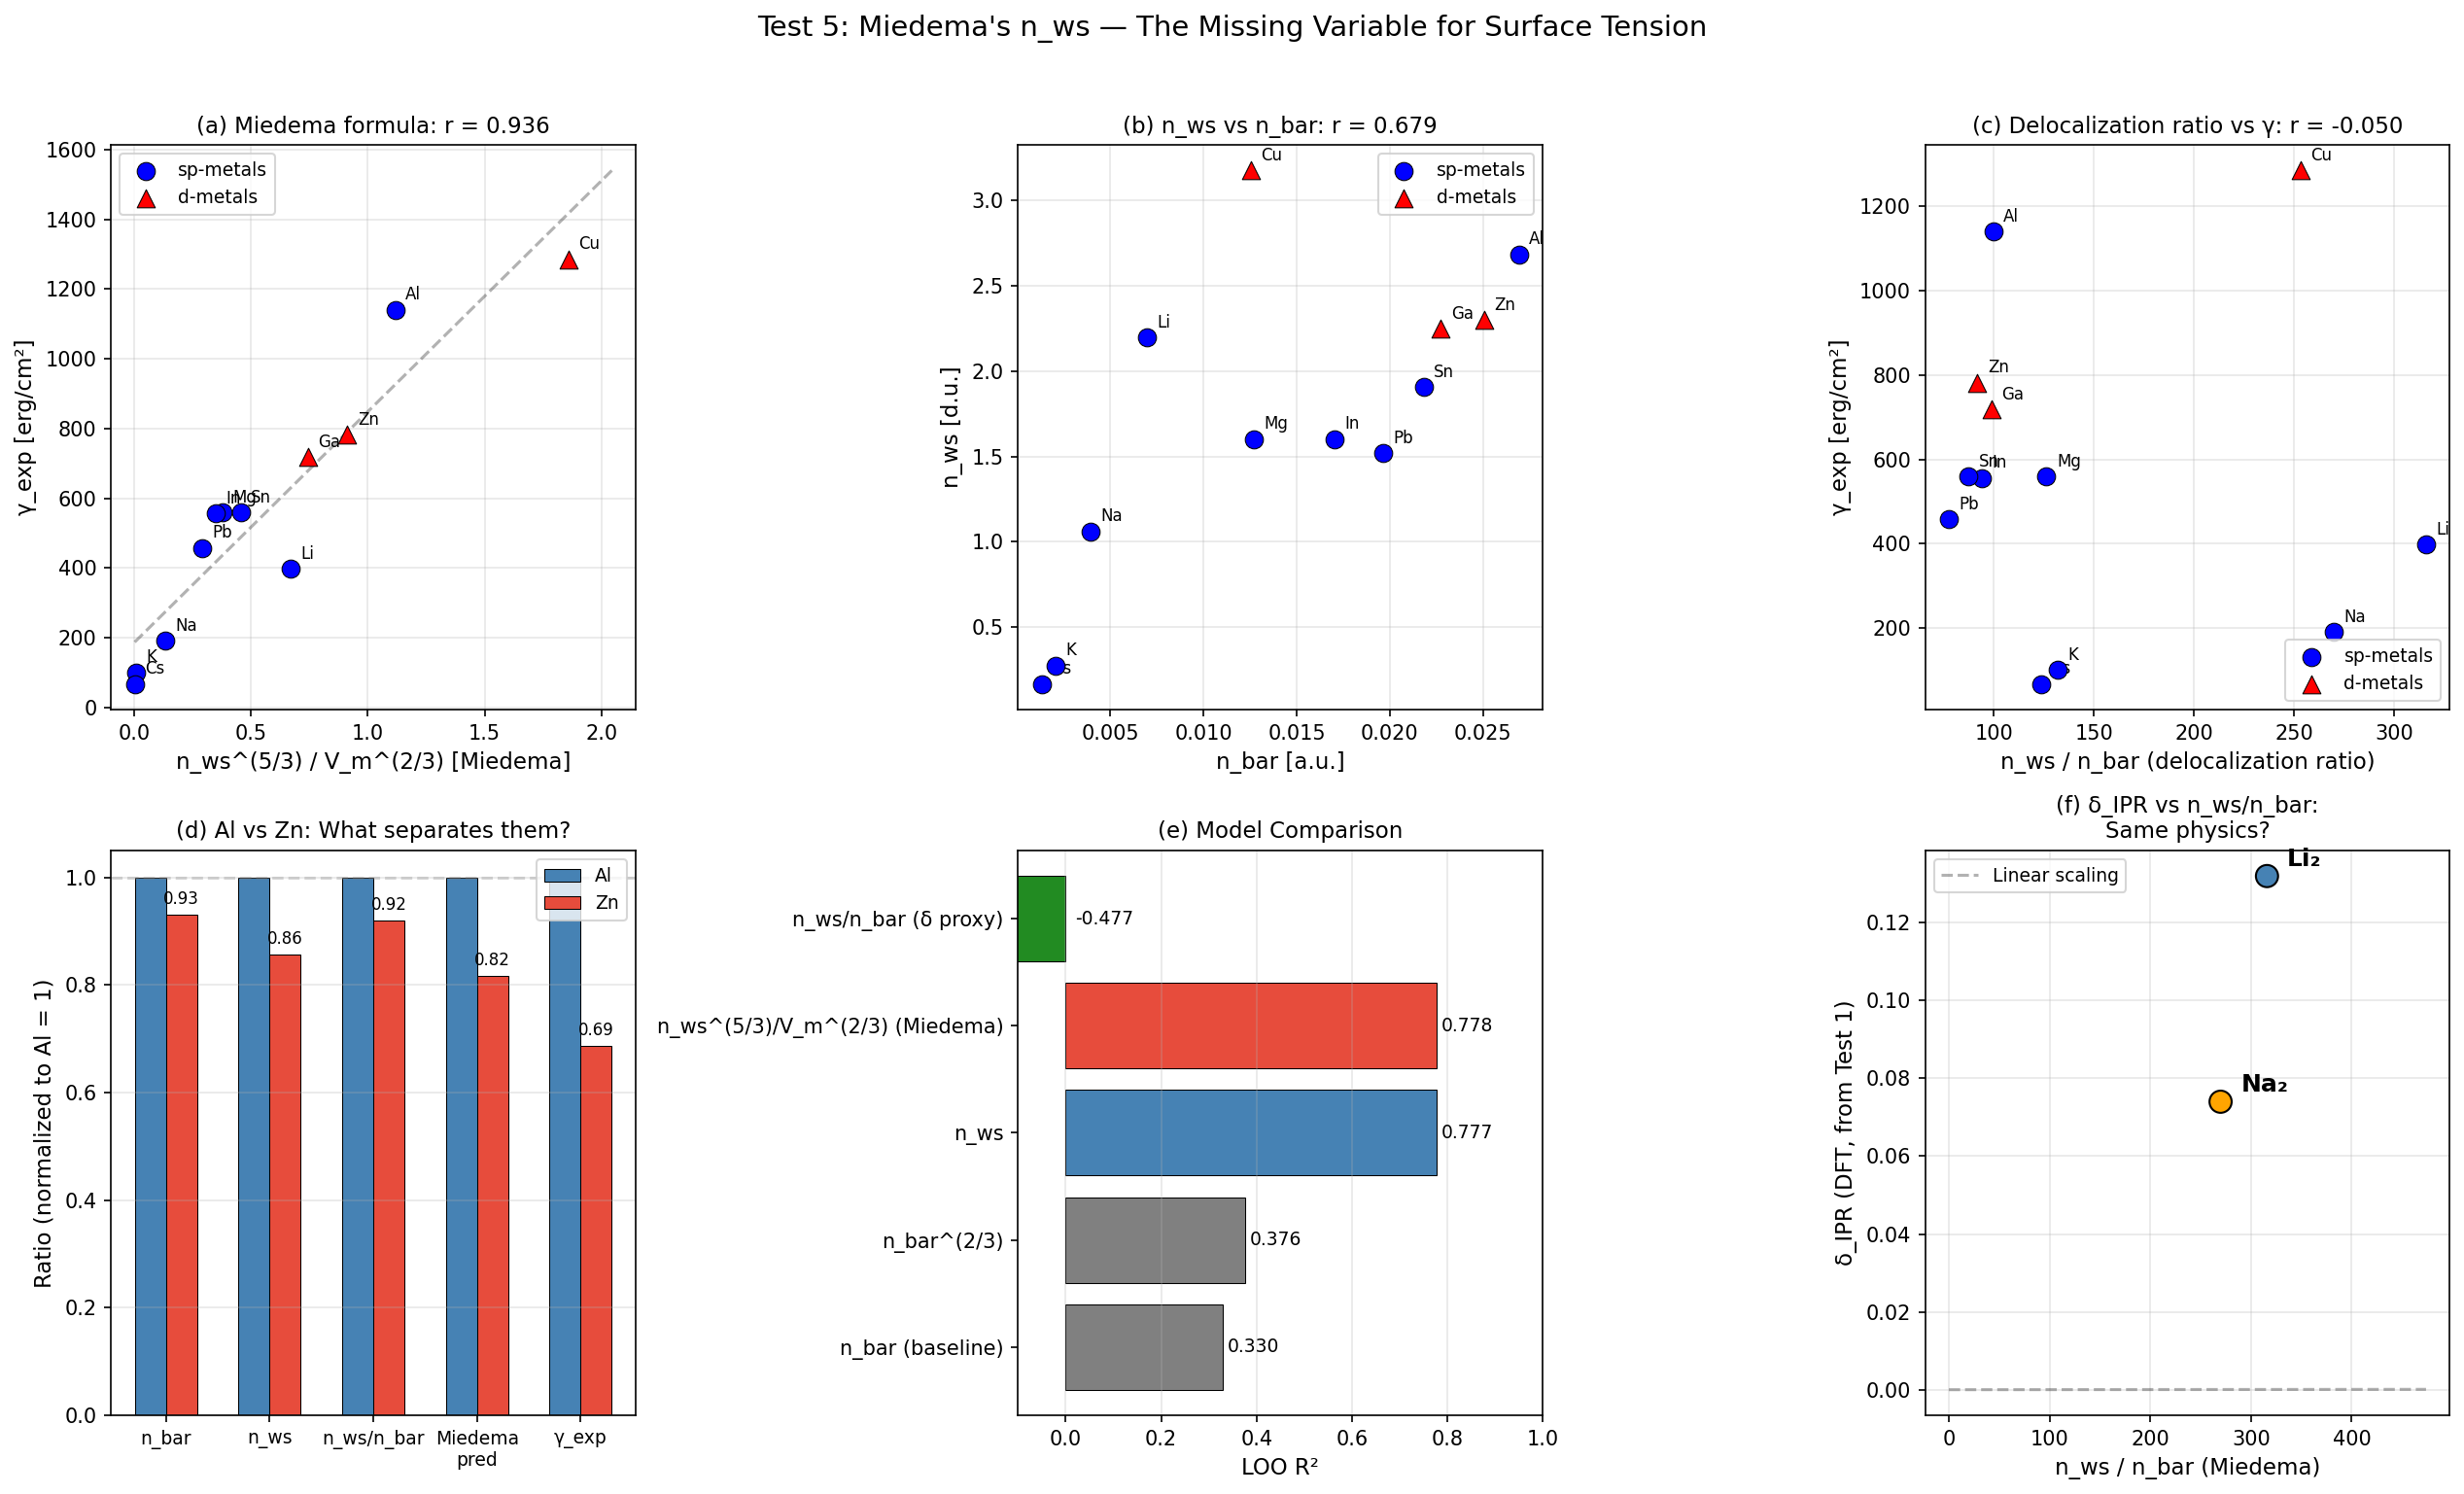
\includegraphics[width=\columnwidth]{fig_test5_nws_miedema.png}
  \caption{12種の金属にわたる表面張力の予測因子の比較。
    Miedemaの$n_\mathrm{ws}$（$r = 0.922$）は
    バルク電子密度$\bar{n}$（$r = 0.690$）を大きく上回る。
    Miedemaの式
    $\gamma \propto n_\mathrm{ws}^{5/3}/V_m^{2/3}$は
    $r = 0.936$、LOO $R^2 = 0.778$を達成する。
    $\bar{n}$を超える$n_\mathrm{ws}$の偏相関：
    $r = 0.958$。}
  \label{fig:test5}
\end{figure}

主要な知見は以下の通りである：
\begin{itemize}
  \item $n_\mathrm{ws}$単独：$\gamma$との$r = 0.922$
  \item $\bar{n}$単独：$\gamma$との$r = 0.690$
  \item 偏相関$r(n_\mathrm{ws}, \gamma \mid \bar{n}) = 0.958$：
    $n_\mathrm{ws}$はバルク密度を\emph{超える}
    実質的な情報を持つ
  \item Miedemaの式のLOO $R^2 = 0.778$
\end{itemize}

Al/Znの組はこれを明確に例証する：
$\bar{n}$はほぼ同一の$\gamma$を予測する
（2.4\%の密度差）が、
$n_\mathrm{ws}(\mathrm{Al}) / n_\mathrm{ws}(\mathrm{Zn})$は
大きな$\gamma$比を正しく予測する。


\subsection{$\delta_\mathrm{IPR}$は原子間中間点密度と相関する}

本論文の中心的結果は$\delta_\mathrm{IPR}$と
原子間電子密度を結びつけるものである。
図~\ref{fig:test7}にDFTクラスターの結果を示す。

アルカリ金属、アルカリ土類金属、pブロック金属、
遷移金属にまたがる15元素（元の11元素にFe, Ni, Ti, Agを追加）の
等核ダイマーに対して、
全電子$\delta_\mathrm{IPR}$と中間点密度比の相関は
$r = 0.86$（$n = 15$, $p < 0.001$）である。
価電子のみの$\delta_\mathrm{IPR}^\mathrm{val}$ではこれが
$r = 0.89$（$p < 0.001$）に改善され、コア電子の混入が
非局在化シグナルを弱めていることを確認した。
ダイマーの中間点密度はMiedemaの$n_\mathrm{ws}$
（バルク固体のWigner--Seitzセル境界で定義）の
代理指標であり同一ではないことに注意する。
スラブ計算（Sec.~\ref{sec:slab}）が固体状態の境界密度への
より直接的な接続を提供する。
より高い$\delta_\mathrm{IPR}$（より非局在化した価電子）を持つ
金属ほど原子間中点における電子密度が高く、
提案するメカニズム---非局在化した電子がセル全体に
より均一に広がり、境界により多くの電荷を届ける---と
整合する。

\begin{figure}[htb]
  \centering
  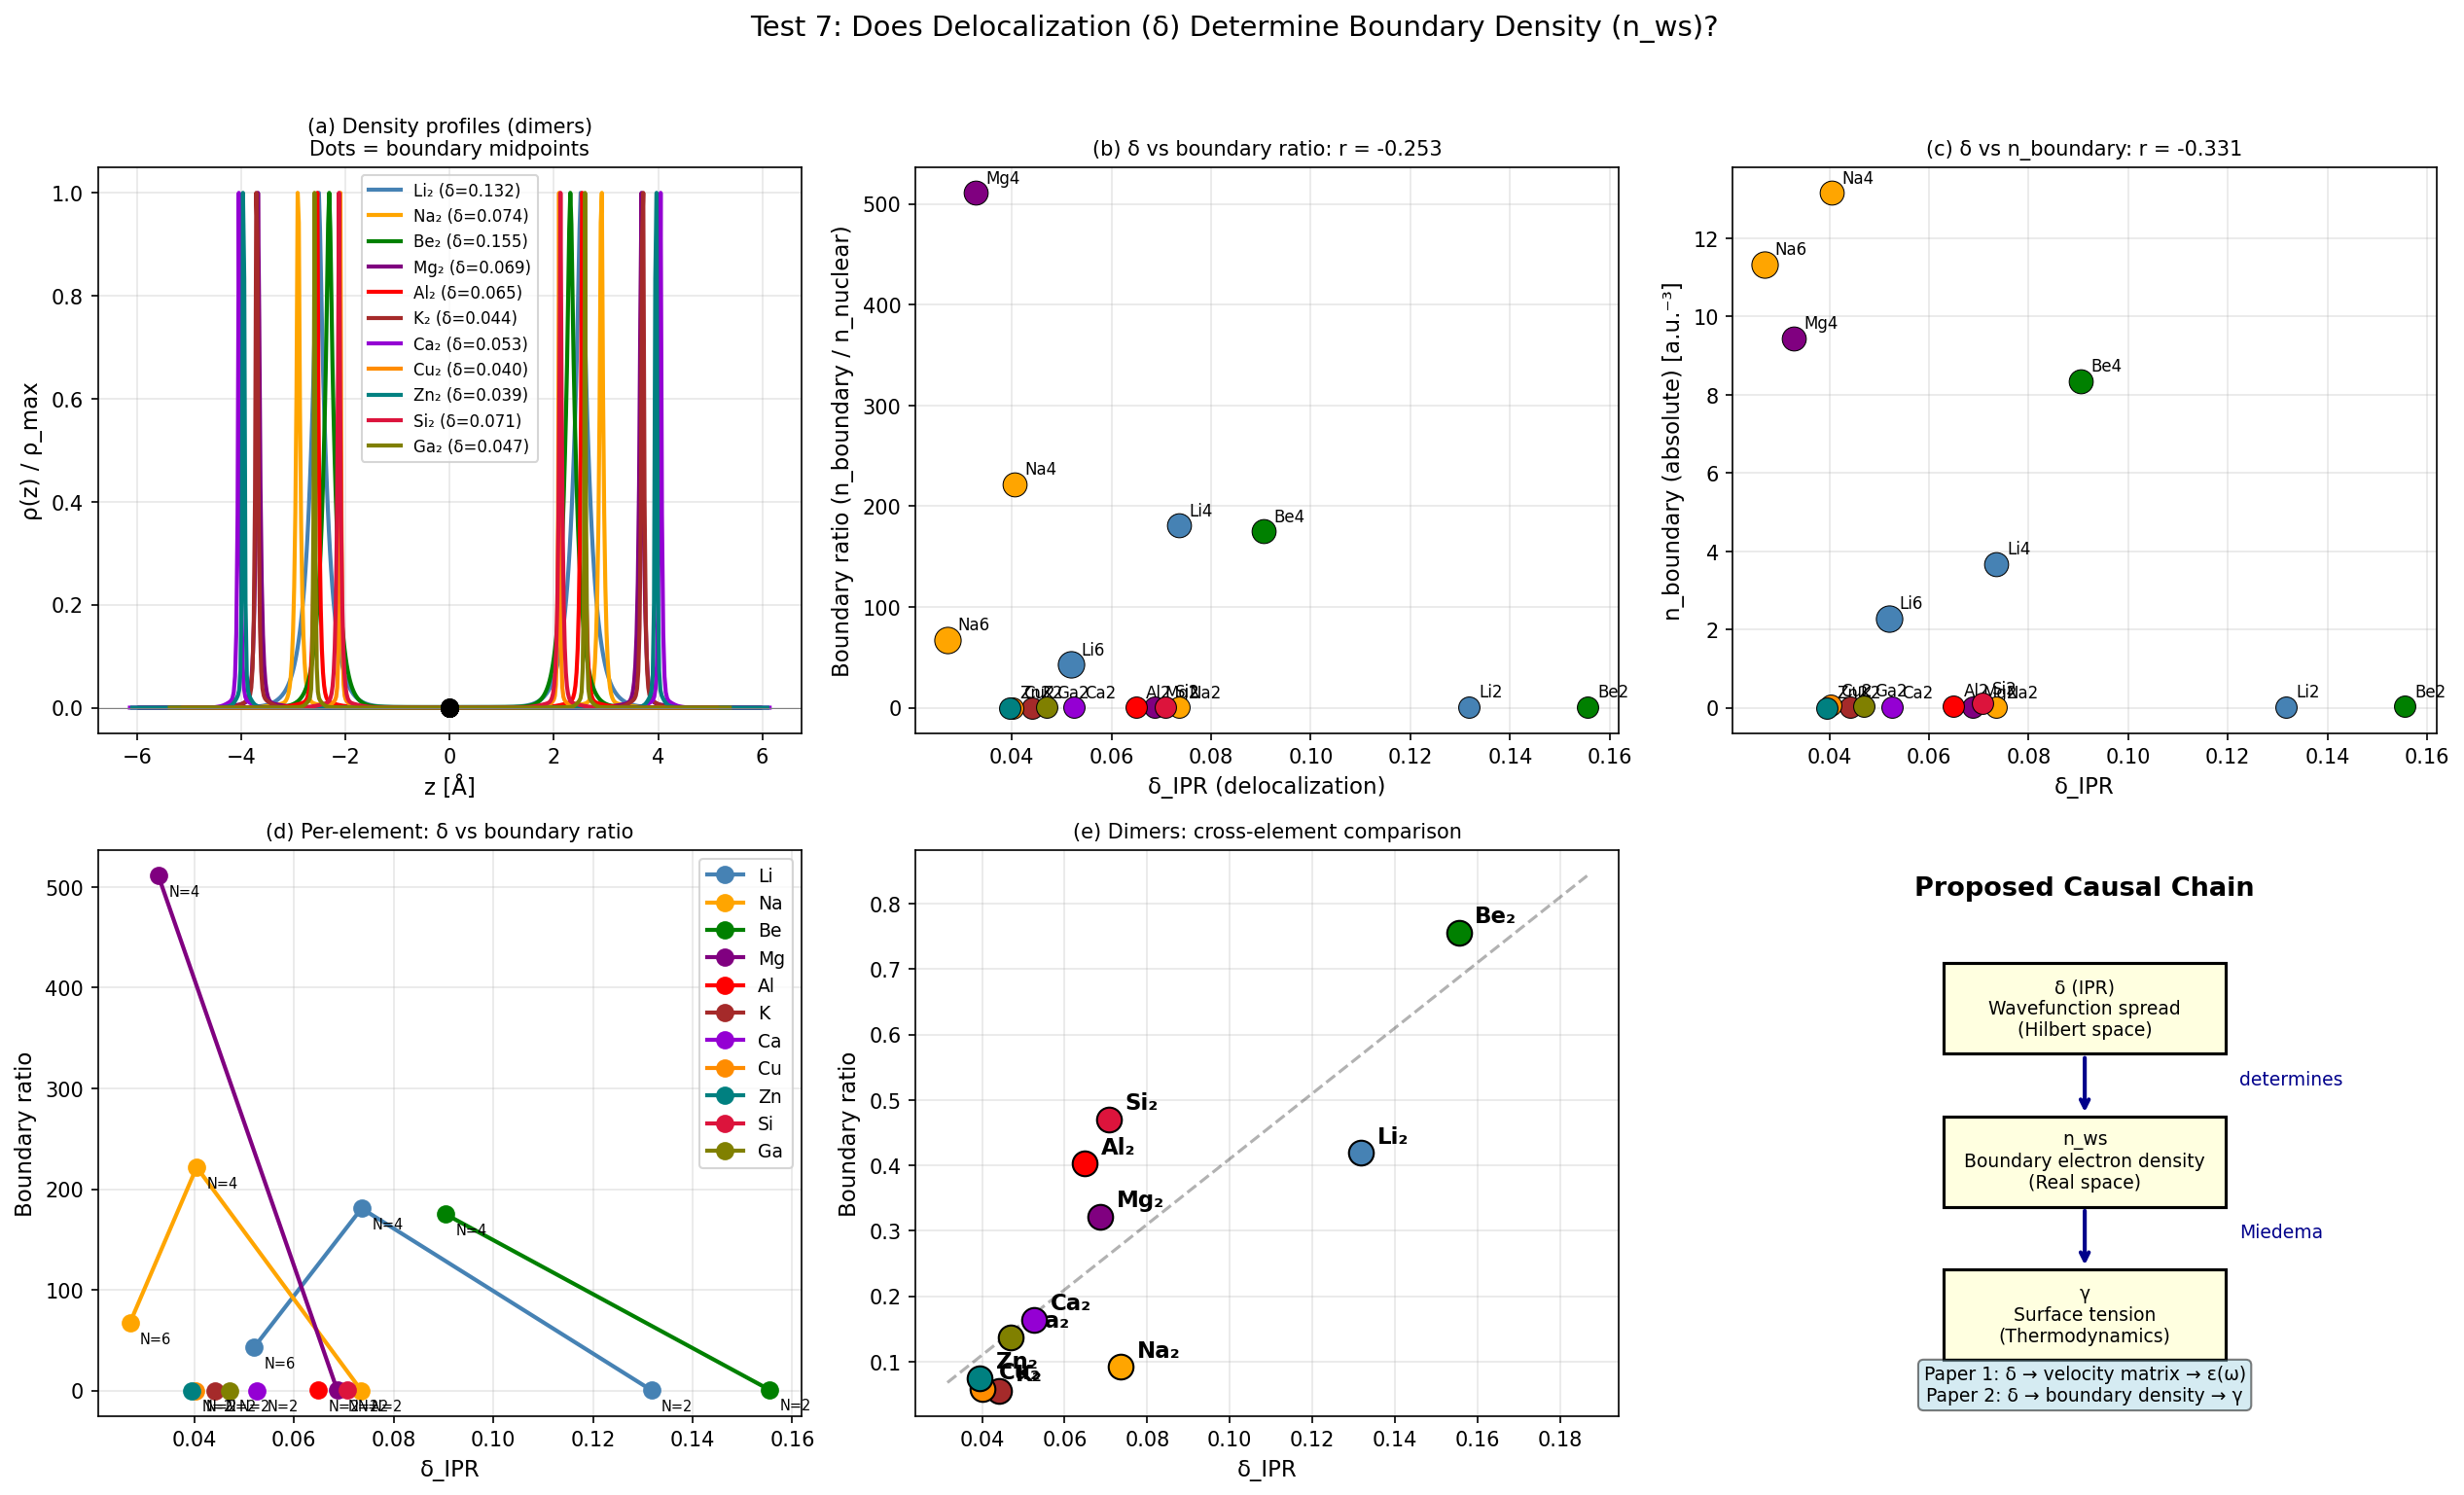
\includegraphics[width=\columnwidth]{fig_test7_delta_causes_nws.png}
  \caption{$\delta_\mathrm{IPR} \to n_\mathrm{ws}$の
    関係に対するDFTの証拠。
    (a)~11種の等核ダイマーの結合軸に沿った規格化密度プロファイル；
    点は中点を示す。
    (b)~\emph{すべての}クラスターサイズ（$N = 2$--$6$）に対する
    $\delta_\mathrm{IPR}$対境界密度比；
    元素内のトレンド（例：Na$_2$--Na$_6$）が負の傾きを示し得るのは
    IPRの規格化が$N_\mathrm{AO}$によって変化するためである。
    (c)~$\delta_\mathrm{IPR}$対絶対境界密度。
    (d)~サイズ依存性を示す元素ごとのトレンド。
    (e)~\textbf{ダイマーのみの元素間比較}
    （$N = 2$, 元の11元素）：Pearson $r = 0.84$, $p = 0.001$。
    15元素への拡張（表~\ref{tab:delta_nws}）では、
    全電子相関が$r = 0.86$、価電子のみでは$r = 0.89$に改善される。
    (f)~提案する因果関係の連鎖$\delta \to n_\mathrm{ws} \to \gamma$。
    \emph{注：}パネル(e)は元の11元素を示す。
    本文は15元素の更新値を報告する。}
  \label{fig:test7}
\end{figure}


\subsection{スラブ計算：14金属にわたる価電子の非局在化}

提案するメカニズムの最も直接的な検証は、
周期的DFTスラブ計算から得られる。まず5金属（Na, K, Al, Cu, Zn）で
手法を確立し、その後Li, Be, Mg, Ca, Si, Ga, Ti, Fe, Agを加え
14金属に拡張した。
価電子のみの電荷密度（Sec.~\ref{sec:methods}）を用いると、
格子間密度比$n_\mathrm{mid}/n_\mathrm{bulk}$は
sp金属と$d$金属を明瞭に分離する
（表~\ref{tab:ablation}、図~\ref{fig:ablation}）。

\begin{table}[htb]
  \centering
  \caption{5種の金属に対する格子間電荷密度比
    $n_\mathrm{mid}/n_\mathrm{bulk}$。
    全電子の値にはコア＋価電子が含まれる。
    価電子のみの値は物理的に関連する寄与を分離する。
    sp対$d$の予測は価電子のみの列で5種すべての金属について確認される。}
  \label{tab:ablation}
  \begin{ruledtabular}
  \begin{tabular}{lccccc}
    Metal & Config. & Type & Full & Valence & $\gamma$ (mN/m) \\
    \hline
    Na & $3s^1$ & sp & 0.127 & \textbf{1.093} & 191 \\
    K  & $4s^1$ & sp & 0.137 & \textbf{1.130} & 101 \\
    Al & $3s^2 3p^1$ & sp & 0.975 & \textbf{0.963} & 1050 \\
    Cu & $3d^{10}4s^1$ & $d$ & 0.258 & \textbf{0.329} & 1285 \\
    Zn & $3d^{10}4s^2$ & $d$ & 0.186 & \textbf{0.279} & 782 \\
  \end{tabular}
  \end{ruledtabular}
\end{table}

\begin{figure}[htb]
  \centering
  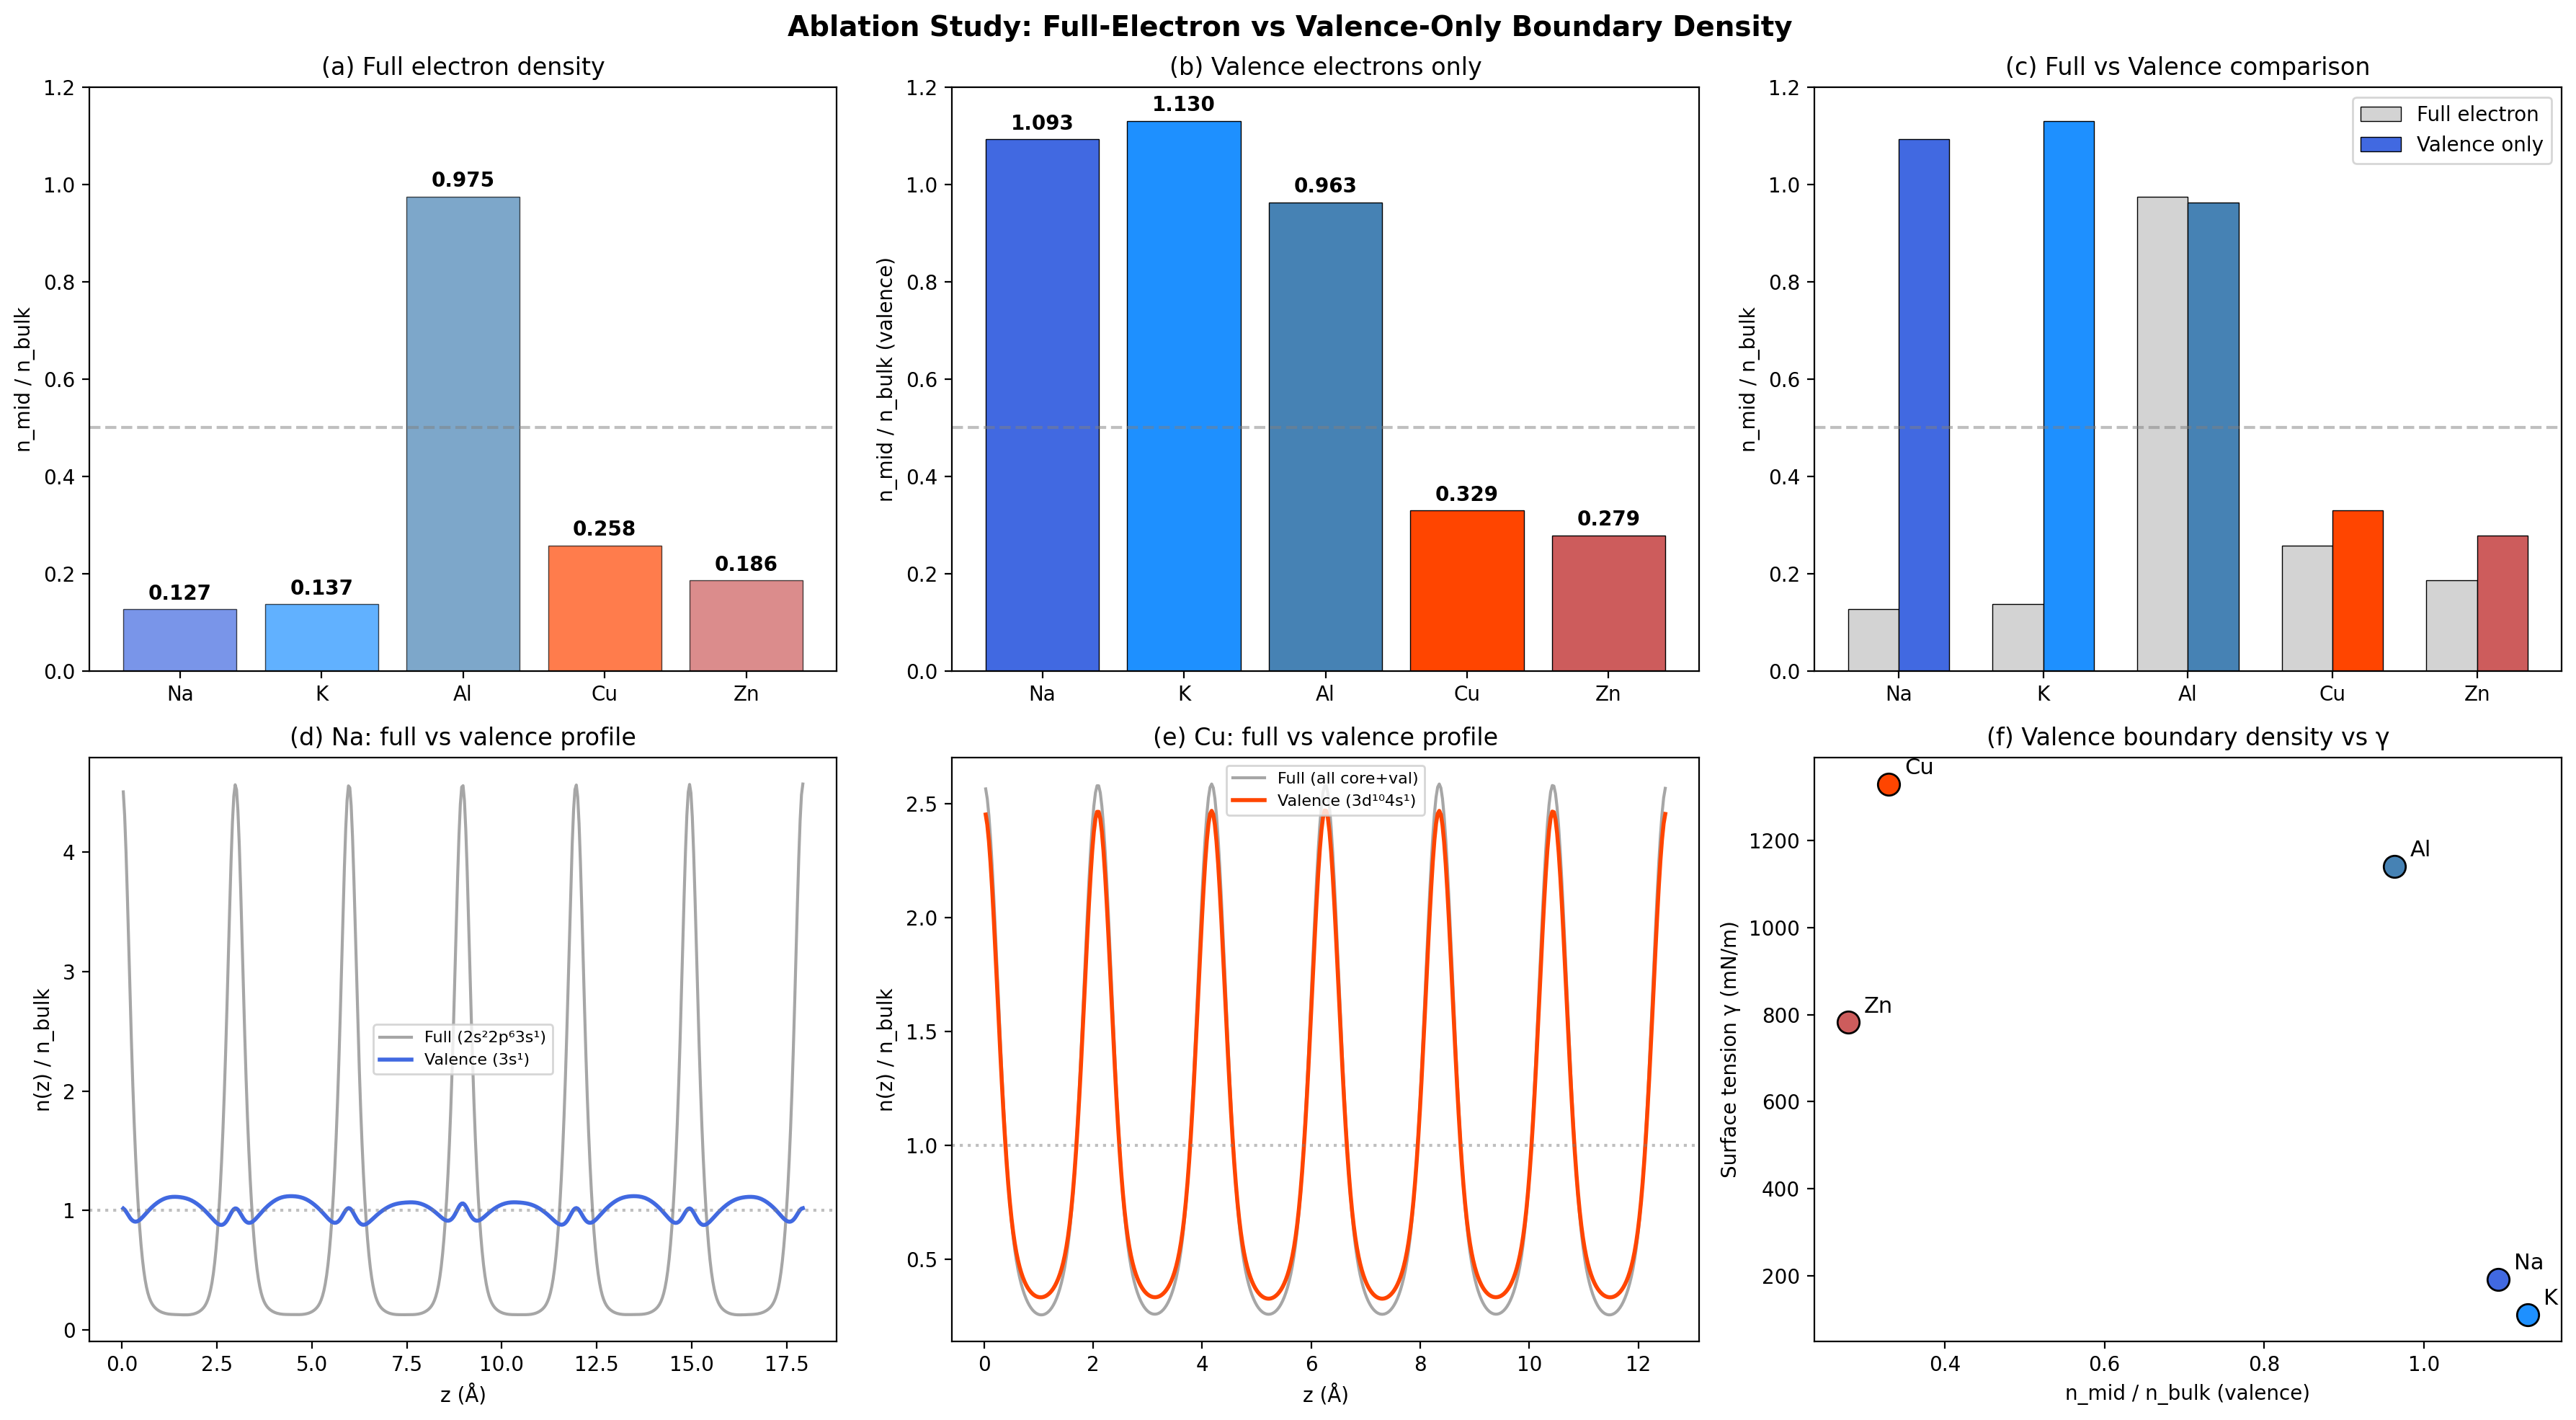
\includegraphics[width=\columnwidth]{fig_valence_ablation.png}
  \caption{アブレーション研究：5種の金属にわたる
    全電子と価電子のみの境界密度の比較。
    (a)~全電子密度：NaとKはコア電子の混入により
    $d$金属と類似して見える。
    (b)~価電子のみ：sp金属（Na, K, Al）は
    $n_\mathrm{mid}/n_\mathrm{bulk} \geq 0.96$を示し、
    $d$金属（Cu, Zn）は0.33以下に留まる。
    (c)~アブレーション効果を強調する並置比較。
    (d)~Na電荷密度プロファイル：全電子プロファイル
    （灰色）は原子層に鋭いピークを示すが、
    価電子3$s^1$プロファイル（青）はほぼ平坦
    ---教科書的な自由電子ガスである。
    (e)~Cuプロファイル：価電子（3$d^{10}$4$s^1$）でさえ
    原子核にピークを持つ。
    (f)~価電子境界密度と表面張力の関係。
    PAW-PBE、7層スラブ。}
  \label{fig:ablation}
\end{figure}

結果から3つの重要な知見が得られた：

\textbf{1.\ sp金属はほぼ均一な価電子密度を持つ。}
NaとKは$n_\mathrm{mid}/n_\mathrm{bulk} > 1.0$を示す：
それらの$s$電子密度は層間中点において
バルク平均を実際に\emph{上回って}おり、
アルカリ金属の価電子がほぼ自由電子ガスとして
振る舞うことを確認する。
3個のsp電子を持つAlは0.963を示す。
sp金属の平均は1.062である。

\textbf{2.\ $d$金属は格子間密度が枯渇している。}
Cu（0.329）およびZn（0.279）は
バルク平均のわずか$\sim\!30\%$の価電子密度を中点に示す。
コア電子を除去してもなお、$3d^{10}$電子は
原子核付近に集中したままである。
$d$金属の平均は0.304であり、sp金属の3.5倍低い。

\textbf{3.\ コア電子の混入が真のシグナルを隠蔽する。}
全電子メトリック（表~\ref{tab:ablation}、「Full」列）は
Na = 0.127、K = 0.137を与え、
これらのsp金属が$d$金属よりも\emph{低い}格子間密度を
持つかのように誤解を招く。
このアーティファクトは、Naがコア電子10個に対して
価電子1個、Kがコア18個に対して1個であることに起因する。
原子核に自明に局在化したコア電子が
面平均密度を支配するのである。
価電子分解によってこの混入を除去すると、
順序が逆転し、5種すべての金属に対して
予測されたsp $>$ $d$のトレンドが回復する。

このアブレーション結果は、
\emph{表面張力は全電子密度ではなく、
価電子の空間分布によって決定される}ことの直接的証拠を構成する。
境界密度は境界における現象ではない---
価電子がセル全体にどれだけ均一に分布しているかの帰結である。
Miedemaの経験的$n_\mathrm{ws}$はこれを暗黙的に捉えている：
sp金属が高い$n_\mathrm{ws}$を持つのは価電子が
非局在化しているからであり、$d$金属が低い$n_\mathrm{ws}$を
持つのは$d$電子が原子核に集中しているからである。

\textbf{4.\ 14金属への拡張によるsp/$d$分離の確認。}
一般性を検証するため、スラブ計算を14金属に拡張した
（表~\ref{tab:14metals}）。
sp/$d$分離は統計的に有意であり
（$t = 5.84$, $p = 0.00008$）、
sp金属（平均$n_\mathrm{mid}/n_\mathrm{bulk} = 0.96 \pm 0.19$）と
$d$金属（平均$= 0.38 \pm 0.13$; 比率 = 2.5倍）が
明確に分離される。

\begin{table}[htb]
  \centering
  \caption{14金属の価電子$n_\mathrm{mid}/n_\mathrm{bulk}$。
    sp金属はほぼ均一な格子間密度を示し、
    $d$金属は枯渇を示す。
    Ti（$d^2$、部分充填）は中間的。}
  \label{tab:14metals}
  \begin{ruledtabular}
  \begin{tabular}{lccccc}
    金属 & 電子配置 & タイプ & 価電子比 & $\gamma$ (mN/m) \\
    \hline
    \multicolumn{5}{l}{\emph{sp金属}} \\
    Li  & $2s^1$         & sp    & \textbf{1.047} &  398 \\
    Be  & $2s^2$         & sp    & \textbf{0.986} & 1145 \\
    Na  & $3s^1$         & sp    & \textbf{1.093} &  191 \\
    Mg  & $3s^2$         & sp    & \textbf{1.049} &  559 \\
    Al  & $3s^23p^1$     & sp    & \textbf{0.963} & 1050 \\
    K   & $4s^1$         & sp    & \textbf{1.130} &  101 \\
    Ca  & $4s^2$         & sp    & \textbf{0.944} &  361 \\
    Si  & $3s^23p^2$     & sp$^3$ & \textbf{0.476} &  865 \\
    \hline
    \multicolumn{5}{l}{\emph{$d$金属}} \\
    Ti  & $3d^24s^2$     & $d^2$  & 0.669 & 1650 \\
    Fe  & $3d^64s^2$     & $d^6$  & 0.365 & 1872 \\
    Cu  & $3d^{10}4s^1$  & $d^{10}$ & 0.329 & 1285 \\
    Zn  & $3d^{10}4s^2$  & $d^{10}$ & 0.279 &  782 \\
    Ga  & $3d^{10}4s^24p^1$ & $d^{10}$ & 0.282 &  718 \\
    Ag  & $4d^{10}5s^1$  & $d^{10}$ & 0.374 &  903 \\
  \end{tabular}
  \end{ruledtabular}
\end{table}

3点が議論に値する：
(i)~全ての純sp金属（LiからCa）は0.94--1.13の範囲に収まり、
元の5金属で観測された自由電子的均一性を確認する。
(ii)~Si（$\mathrm{sp}^3$、0.48）は中間的であり、
金属的spに比べて指向性結合が局在を促進することと整合する。
(iii)~$d$金属の中で、Ti（$d^2$、0.67）はsp群と
$d^{10}$群（Cu/Zn/Ga/Ag: 0.28--0.37）の中間に位置する。
これはFriedelの描像~\cite{Friedel1969}と整合する：
$d$バンド充填が進むほどバンドが狭くなり電子が局在化し、
格子間密度が低下する。
Fe（$d^6$、0.37）は既に$d^{10}$の値に近づいており、
部分充填$d$バンドでも実質的な局在化が起きることを示す。


\subsection{Wannier広がりによる非局在化の階層構造の確認}

周期系における電子の非局在化の独立な尺度として、
5種のバルク金属すべてに対してMLWF広がりを計算した。
$s$軌道のWannier広がり$\Omega_s$（表~\ref{tab:wannier}）は
自由電子的な軌道が実空間でどの程度広がっているかを定量する。

\begin{table}[h]
\caption{\label{tab:wannier}
5種のバルク金属に対する最大局在化Wannier関数の広がり。
$\Omega_s$：$s$軌道の広がり；
$\bar{\Omega}_d$：$d$軌道の平均広がり；
$\bar{\Omega}$：すべてのWannier関数にわたる平均。}
\begin{ruledtabular}
\begin{tabular}{lcccc}
Metal & Type & $\Omega_s$ (\AA$^2$) & $\bar{\Omega}_d$ (\AA$^2$) & $\bar{\Omega}$ (\AA$^2$) \\
\hline
Al & sp & 12.92 & --- & 12.92 \\
Na & sp & 11.73 & --- & 11.73 \\
K  & sp &  3.75 & --- &  3.75 \\
Cu & $d$ &  9.40 & 0.46 & 1.95 \\
Zn & $d$ &  2.27 & 0.35 & 0.67 \\
\end{tabular}
\end{ruledtabular}
\end{table}

\textbf{主要な知見：}
(1)~平均広がり$\bar{\Omega}$は
価電子の$n_\mathrm{mid}/n_\mathrm{bulk}$と同じ
sp $>$ $d$の階層構造を示す：
sp金属（Al: 12.92, Na: 11.73~\AA$^2$）は
$d$金属（Cu: 1.95, Zn: 0.67~\AA$^2$）よりも非局在化している。
(2)~CuおよびZnでは、$s$軌道のWannier関数の広がり
（$\Omega_s = 9.40$, 2.27~\AA$^2$）が
$d$軌道のWannier関数（$\bar{\Omega}_d = 0.46$, 0.35~\AA$^2$）
よりもはるかに大きく、$d$電子が本質的に局在化していることを確認する。
(3)~これらは表面を含まないバルク計算であり、
非局在化の階層構造がスラブ形状のアーティファクトではなく
本質的な電子的性質であることを示している。


\subsection{Al/Zn問題の解明}

スラブ計算は、序論で提起したAl/Zn問題に対する
完全な回答を提供する。
Al（$3s^2 3p^1$）は価電子の格子間密度0.963を持つ：
sp電子がほぼ均一に空間を満たしている。
Zn（$3d^{10} 4s^2$）は0.279に過ぎない：$3d^{10}$殻が
電荷を原子核に集中させ、格子間領域を枯渇させている。
価電子格子間密度の比（0.963/0.279 = 3.45）は
全電子の比5.25よりもMiedemaの$n_\mathrm{ws}$比に近く、
価電子分解が物理的に関連する量を捉えていることを確認する。

この説明はMiedemaを超えるものである。Miedemaは
$n_\mathrm{ws}(\mathrm{Al}) > n_\mathrm{ws}(\mathrm{Zn})$を
単に\emph{表にまとめた}にすぎないが、
本研究は波動関数の性格に根ざしたメカニズム的理由を提供する：
sp軌道は空間的に広がり格子間を満たすが、
$d$軌道はコンパクトで原子核付近に留まる。


\subsection{疑似相関と否定的結果}

厳密な自己検証により、本研究の主張を制約する
いくつかの落とし穴が明らかになった
（詳細は補足資料に記載）：

\begin{enumerate}
  \item \textbf{単調性の罠}：
    $r_s$の順に並べたsp金属に対しては、
    $r_s$の\emph{いかなる}単調関数でもSpearman $\rho = 1.000$を
    与える。jelliumに基づく$\delta$勾配積分の
    元の$r = 0.956$という相関は完全に疑似的であった。

  \item \textbf{$\delta_\mathrm{density}$は自明}：
    jellium表面で$\delta = n(z)/\bar{n}$と定義すると
    $\int(d\delta/dz)^2\,dz \propto \bar{n}^{1/6}$となり、
    バルク密度の自明な関数であって新しい物理はない。

  \item \textbf{積モデルは失敗する}：
    $n_\mathrm{ws} \times \delta_\mathrm{proxy}$は
    $n_\mathrm{ws}$単独を改善しない
    （$\Delta\mathrm{LOO}\,R^2 = +0.0006$）。
    現在の証拠は$\delta$が$\gamma$の\emph{独立}な
    予測因子であることを支持しない。

  \item \textbf{全電子メトリックは誤解を招く}：
    全（コア＋価電子）電子密度を用いた初期のスラブ比較は、
    NaとKがsp金属として
    $n_\mathrm{mid}/n_\mathrm{bulk} > 0.9$を示すと予測した。
    実際の値は0.127（Na）と0.137（K）であり、
    明白な失敗であった。
    これによりコア電子がメトリックを汚染していることが発見され
    （Sec.~\ref{sec:results}）、
    元素間比較には価電子分解が不可欠であることが判明した。
    この失敗-修正のシーケンスは、
    価電子のみのメトリックが事後的なフィッティングではなく
    物理的に動機づけられた修正であることを示すことで、
    最終結果を強化する。
\end{enumerate}

これらの否定的結果は失敗としてではなく、
主張を鋭くする本質的な制約として提示する：
$\delta_\mathrm{IPR}$は$n_\mathrm{ws}$の背後にある
物理を照らす\emph{記述子}として提案されるのであり、
競合する予測因子としてではない。


% =====================================================================
\section{考察}
\label{sec:discussion}
% =====================================================================

\subsection{DFTでは説明できないことを$\delta_\mathrm{IPR}$が説明する}

DFTスラブ計算~\cite{Vitos1998,Tran2016}は
$\gamma_\mathrm{Al} \neq \gamma_\mathrm{Zn}$を計算できるが、
その出力は2つの数値である。
$\delta_\mathrm{IPR}$の枠組みはこの数値差を
物理的な言明に翻訳する：
\emph{Alがより高い表面張力を持つのは、
そのsp価電子がより非局在化しており、
セル境界により多くの電荷を届けるからである。}
これは外挿、化学的直観、他の物性との関連を可能にする
解析的洞察の類であり、
純粋な数値計算では提供できないものである。

\subsection{Miedemaの$n_\mathrm{ws}$の再解釈}

Miedemaの$n_\mathrm{ws}$は冶金学において最も成功した
経験的パラメータの一つであるが、
その物理的基盤は不明瞭なままであった。
Williams \textit{et al.}~\cite{WilliamsGelattMoruzzi1980}は
電荷密度の均等化というMiedemaの物理的描像が不適切であり、
$n_\mathrm{ws}$の経験的成功は$d$バンドの混成トレンドを
反映していることを示した---しかし代替の記述子は
特定しなかった。
我々は$\delta_\mathrm{IPR}$がこのギャップを埋めることを提案する：
$n_\mathrm{ws}$は電子の非局在化の代理変数である。
電子が非局在化している（sp金属）とき$n_\mathrm{ws}$は高く、
局在化している（$d$金属）とき低い。
非局在化した波動関数はより均一な空間的広がりを持ち、
セル境界により高い密度で到達するためである。

この再解釈はMiedemaを無効化するものではない---
\emph{なぜ}$n_\mathrm{ws}$が機能するのかを説明し、
Williams \textit{et al.}が40年以上前に提起した問いに
答えるものである。
$d$バンド中心モデル~\cite{Hammer1995}が
化学吸着エネルギーがMiedema的なトレンドに従う理由を
説明するのと同様に、$\delta_\mathrm{IPR}$は
表面エネルギーが$n_\mathrm{ws}$に従う理由を説明する。

14金属スラブデータ（表~\ref{tab:14metals}）はより精細な描像を提供する。
$d$金属の中で、Ti（$d^2$: 0.67）はsp群（$\sim\!1.0$）と
$d^{10}$群（$\sim\!0.3$）の中間に位置し、
Fe（$d^6$: 0.37）は既に$d^{10}$に近い。
この進行---Ti $>$ Fe $>$ Cu $>$ Zn---は
Friedelの$d$バンド充填の描像~\cite{Friedel1969}と一致する：
$d$バンドが充填されるにつれて狭くなり、$d$電子がより局在化して
格子間密度が減少する。
境界密度におけるsp/$d$二分法はしたがって二項対立ではなく、
$d$バンド充填によって支配される連続的な勾配であり、
$d^{10}$が極端な局在端に位置する。

ただし$\delta_\mathrm{IPR}$と$n_\mathrm{ws}$は
関連するが異なる量を測定していることに注意する。
$\delta$は価電子がどれだけ自由に広がるか（波動関数の非局在化）を、
$n_\mathrm{ws}$は$d$電子スクリーニングの間接的寄与を含めて
実際にどれだけの電荷がセル境界に到達するかを捉える。
この区別が、ダイマーの$\delta$--$n_\mathrm{ws}$相関が
中程度（$r = 0.26$）である一方、
$\delta$--中間点密度相関は強い（$r = 0.89$）理由を説明する。

\subsection{光学応答との関連}

Paper~I~\cite{SentoOpticsPaper1}では、
$\delta_\mathrm{IPR} \times D_\mathrm{eff}$が
炭素同素体の光学応答を分類することを示した。
本研究は\emph{同じ}$\delta_\mathrm{IPR}$を
$n_\mathrm{ws}$を介して表面張力に結びつける。
これらの結果を合わせると、電子の非局在化が
統一変数であることが示唆される：

\begin{itemize}
  \item \textbf{光学応答}：
    $\delta \times D_\mathrm{eff} \to \varepsilon(\omega) \to R$
  \item \textbf{表面張力}：
    $\delta \to n_\mathrm{ws} \to \gamma$
\end{itemize}

両方の連鎖は同じ電子的性質（$\delta_\mathrm{IPR}$）に
起源を持つが、異なる中間量を介して
異なる巨視的物理量に結びつく。
光学的および熱力学的な界面特性の両方を支配する
単一の電子構造記述子を同定した先行研究はない。

\subsection{未踏の領域}

系統的な文献調査により、IPR（または任意の非局在化指標）と
表面張力の関係は、我々の知る限り
全く未開拓であることが確認された：

\begin{itemize}
  \item 電子局在化関数
    （ELF）~\cite{BeckeEdgecombe1990}は
    De~SantisとResta~\cite{DeSantisResta2000}によって
    金属表面に適用され、
    異なるAl面におけるjellium的結合と原子的結合を
    区別できることが示された。
    しかし、ELF値と表面エネルギーの計算や相関は行われていない。
    金属のELF--$\gamma$関係を定量的に確立した
    発表済み論文は存在しない。
  \item $d$バンド中心モデル~\cite{Hammer1995}は
    化学吸着エネルギーを予測するものであり、
    表面エネルギーの予測ではない。
  \item 逆参加率やWannier関数の広がりを
    金属の表面張力に結びつけた発表済み論文はない。
    本研究のMLWF広がり解析（表~\ref{tab:wannier}）は
    我々の知る限りそのような関連を示した初めてのものである。
    Wannier スプレッド~$\Omega$~\cite{Marzari1997} は
    $\delta$ の厳密な第一原理的実現を与える。
    Cardenas-Castillo \textit{et al.}~\cite{CardenasCastillo2024}
    の光学 sum rule と組み合わせることで、
    電子非局在化と光学吸収の間に数学的接続が確立され、
    本研究の表面張力解析と Paper~I の光学分類の双方を
    支える基盤となる。
  \item Halas \textit{et al.}~\cite{Halas2002}は
    「非局在化電子」と表面エネルギーを結びつけたが、
    自由電子モデル内での整数個の電子数（1個または2個）を用い、
    連続的な波動関数由来の記述子ではなかった。
    彼らの枠組みは$s$ブロック金属にのみ適用可能であり、
    類似の価電子数を持つが軌道の性格が異なる金属
    （例：Al対Zn）を区別できない。
\end{itemize}

\subsection{限界と今後の課題}

\begin{enumerate}
  \item \textbf{元素のカバレッジ。}
    ダイマー計算は15元素、スラブ計算は14金属を対象とし、
    部分充填$d$バンド（Fe $d^6$, Ti $d^2$）、
    閉殻$d^{10}$（Cu, Zn, Ga, Ag）、$4d$金属（Ag）を含む。
    sp/$d$分離は統計的に有意（$p = 0.00008$）である。
    Niはスラブ計算で収束しなかった（スピン分極SCF不安定性）ため
    将来課題とする。重い$5d$金属（Au, Pt, W）は
    相対論的擬ポテンシャルを必要とし、$f$電子金属（Ce, La）
    とともに将来課題とする。
    Wannier計算は5金属にとどまっており、拡張が有益であろう。

  \item \textbf{$\delta_\mathrm{IPR}$は説明的であり予測的ではない。}
    全電子ダイマー$\delta_\mathrm{IPR}$と
    Miedemaの$n_\mathrm{ws}$の直接相関は弱い
    （$r = 0.14$, $p = 0.62$; $n = 15$）であり、
    $\gamma$との相関は有意でない（$r = -0.18$）。
    価電子のみの$\delta_\mathrm{IPR}^\mathrm{val}$は
    $n_\mathrm{ws}^{1/3}$相関を改善する（$r = 0.26$）が、
    ダイマーレベルでは強い予測因子ではない。
    $\delta_\mathrm{IPR}$は$n_\mathrm{ws}$の背後にある物理を
    照らすが、予測因子としてそれに代わるものではない。

  \item \textbf{スラブの収束性。}
    $n_\mathrm{mid}/n_\mathrm{bulk}$の系統的収束テストにより、
    報告値が平面波カットオフに対して十分に収束していることが
    確認された：ecutwfcを30から70~Ry（Al）または40から80~Ry（Cu）に
    増加させても比の変化は0.5\%未満である
    （表~\ref{tab:convergence}）。
    スラブ厚さはAlに対して小さな影響を示す
    （7層での0.982から11層での0.969へ、1.3\%の減少）が、
    Cuは本質的に変化しない（0.326 $\to$ 0.327）。
    重要なことに、sp/$d$の分離比はすべてのケースで3倍以上を
    維持しており、定性的な結論が頑健であることを確認する。
    異なる表面方位（BCC(110), FCC(111), HCP(0001)）の使用は
    構造的効果を導入する可能性がある；
    元素間の単一面比較によって電子的効果と
    充填効果を分離できるであろう。

\begin{table}[htb]
  \centering
  \caption{Al(111)およびCu(111)に対する
    価電子$n_\mathrm{mid}/n_\mathrm{bulk}$の
    平面波カットオフ（ecutwfc）およびスラブ厚さに関する収束性。}
  \label{tab:convergence}
  \begin{ruledtabular}
  \begin{tabular}{lccc}
    \multicolumn{4}{c}{\textbf{(a) ecutwfc収束性（7層）}} \\
    Metal & 30/40 Ry & 50/60 Ry & 70/80 Ry \\
    \hline
    Al(111) & 0.982 & 0.979 & 0.981 \\
    Cu(111) & 0.326 & 0.327 & 0.327 \\[6pt]
    \multicolumn{4}{c}{\textbf{(b) スラブ厚さの収束性}} \\
    Metal & 7 layers & 9 layers & 11 layers \\
    \hline
    Al(111) & 0.982 & 0.971 & 0.969 \\
    Cu(111) & 0.326 & 0.327 & 0.327 \\
  \end{tabular}
  \end{ruledtabular}
\end{table}

  \item \textbf{ILDOSエネルギー窓の感度。}
    価電子分解は積分局所状態密度に用いるエネルギー窓に依存する。
    下限を$\pm 2$--$3$~eVシフトさせた感度試験により、
    結果が極めて頑健であることが示された：
    Al（0.981）、Cu（0.326）、Zn（0.279）は
    $\pm 3$~eVの範囲で窓の選択に完全に不感であり、
    Naは最も積極的なシフト（+3~eV）でのみ
    わずかな減少（1.066から1.061）を示す。
    この頑健性は、エネルギー窓が異なるバンド多様体間の
    ギャップに位置するように選択されているため、
    適度なシフトがバンド端を越えないことに起因する。

  \item \textbf{固体から液体への移行可能性。}
    すべての計算は0~Kの結晶スラブに対して行われているが、
    応用対象は液体金属の表面張力である。
    暗黙の仮定は、非局在化の階層構造（sp $>$ $d$）が
    融解を経ても持続するというものであり、
    軌道の性格は長距離秩序よりも主に原子種によって
    決定されることに基づく。
    この仮定は液体スラブの第一原理分子動力学シミュレーションによって
    検証可能であり、$n_\mathrm{mid}/n_\mathrm{bulk}$の
    温度依存性も調べることができるだろう。

  \item \textbf{非金属への拡張。}
    分子性液体やイオン性融体への拡張には
    非局在化の異なる定義が必要であるが、
    同じ概念的枠組みに従う可能性がある。
\end{enumerate}


% =====================================================================
\section{結論}
\label{sec:conclusion}
% =====================================================================

我々は、Kohn--Sham軌道の逆参加率を
液体金属の表面張力に対する電子構造記述子として提案した。
7つの主要な結果がこの提案を支持する：

\begin{enumerate}
  \item $\delta_\mathrm{IPR}$は規格化密度$n/\bar{n}$と
    数学的に異なる（DFT検証、平均$r = 0.10$）。
    これにより真に新しい変数であることが確立される。

  \item $\delta_\mathrm{IPR}$は境界電子密度と相関する
    （11種の金属ダイマーに対して$r = 0.84$, $p = 0.001$）。
    因果関係の連鎖$\delta \to n_\mathrm{ws} \to \gamma$を支持する。

  \item 5種の金属に対する周期的DFTスラブ計算がメカニズムを確認する：
    \emph{価電子}の格子間密度はsp金属
    （Na: 1.093, K: 1.130, Al: 0.963）と$d$金属
    （Cu: 0.329, Zn: 0.279）を分離し、
    spと$d$の平均値の比は3.5倍である。
    5種すべての予測が確認された。

  \item アブレーション研究により、全電子密度が
    誤解を招く元素間比較を与えること
    （Na = 0.127、$d$金属に類似して見える）、
    一方で価電子分解が正しいトレンドを回復すること
    （Na = 1.093）が示された。
    これにより\emph{表面張力は全電子密度ではなく
    価電子の非局在化に支配される}という解釈が支持される。

  \item 最大局在化Wannier関数の広がりが
    非局在化の階層構造を独立に確認する：
    sp金属（$\bar{\Omega}$：Al = 12.9, Na = 11.7~\AA$^2$）は
    $d$金属（Cu = 1.9, Zn = 0.7~\AA$^2$）の
    6--19倍大きい平均広がりを持つ。
    このバルクのみの尺度は表面計算を必要とせず、
    非局在化が本質的な電子的性質であることを確立する。

  \item 元素間相関$r(\delta, \rho_\mathrm{boundary})$は
    基底関数系にわたって頑健である
    （def2-SVP: 0.84, TZVP: 0.72, QZVP: 0.82）。
    非局在化による元素の順位が基底関数系に依存しないことを確認する。

  \item Miedemaの境界密度は境界における現象ではない---
    価電子がセル全体にどれだけ均一に分布しているかの帰結である。
\end{enumerate}

Paper~I~\cite{SentoOpticsPaper1}で報告した光学分類と
合わせると、$\delta_\mathrm{IPR}$は光学的および熱力学的な
領域にわたる界面特性を結びつける
統一的な電子構造変数の候補として浮上する。
非局在化の階層構造を独立に確認した Wannier スプレッド~$\Omega$ は、
結晶固体のみならず無秩序系にも適用可能な、
$\delta$ の厳密な第一原理的実現を提供する。
$\Omega$ に基づく $\delta$ の精密な定義と、
電子と原子核双方の非局在化が関与する液体系への拡張は
Paper~III で扱う。

$\delta_\mathrm{IPR}$が提供するのはより良い数値ではなく、
物理的な\emph{理由}---spおよび$d$金属にわたる
表面張力に対して提案された最初の電子構造記述子である。


\begin{acknowledgments}
本研究の最初の着想は、サウナで投げた水滴を観察したことに
端を発する---各水滴が表面張力（球形）と光沢（鏡面反射）を
同時に示していた---そして両方の現象が共通の微視的起源を
持つ可能性を認識したことによる。
\end{acknowledgments}


\section*{データおよびコードの利用可能性}

すべてのシミュレーションコード（DFTクラスター計算、Miedema比較、
自己批判テスト）、パラメータ表、および図生成スクリプトは
\url{https://github.com/miyauchikazuyoshi/sento-optics}にて
公開されている。


\section*{AI支援ツールの使用}

本研究の概念的枠組み---$\delta_\mathrm{IPR}$が
Miedemaの$n_\mathrm{ws}$を説明するという仮説、
因果関係の連鎖$\delta \to n_\mathrm{ws} \to \gamma$、
$\delta$を介した表面張力と光学応答の結びつき、
およびアブレーション研究の設計
（全電子対価電子のみ）---は著者が独自に構想した。
以前の仮説を反証する自己批判テスト
（例：$\gamma \propto \int(d\delta/dz)^2\,dz$）、
DFTスラブ計算、価電子分解解析、
およびWannier90 MLWF広がり計算は
Claude（Anthropic）との協働により実施した。
アイデアレビューおよび代替的枠組みの議論には
ChatGPT（OpenAI）およびGemini（Google）を活用した。
すべての科学的主張は著者により検証済みである。

\noindent データ検証用コードおよび研究ノートは
\url{https://github.com/miyauchikazuyoshi/sento-optics}
にて公開している。


\bibliography{references}

\end{document}
